\documentclass{article}
\usepackage[utf8]{inputenc}
\usepackage{graphicx}
\usepackage{tabu}
\usepackage[spanish]{babel}

\begin{document}
\begin{figure}[t!]

\includegraphics[scale=0.3]{logo_udp.PNG}
\label{fig:udplogo}
\end{figure}

\title{\textbf{{Laboratorio 4 \\ Spanning Tree Protocol y Virtual LAN \vspace{10cm}}}}
\author{\hspace{8cm} Vicente Henriquez \\ \hspace{8cm} Franco Montenegro}
\date{\hspace{8cm} 26/09/2017}

\maketitle
\newpage

\tableofcontents
\newpage
\section{Introducción\vspace{0.5cm}}
En este laboratorio se trabajará con dos herramientas fundamentales para el funcionamiento de las redes, el STP (Spanning Tree Protocol) y Vlan (Virtual Local Area Network), que consisten en detectar posibles bucles para la transmisión en la red con objeto de evitarlos y separar, a nivel lógico, las redes LAN respectivamente. Se buscará entender el funcionamiento del STP y aprender a configurar e implementar las VLANs para así comprender las ventajas y desventajas que puedan tener.
\newpage
\section{Desarrollo\vspace{0.5cm}}
\subsection{Actividad 1\vspace{0.3cm}}
Se analizarán los efectos de una red con topología malla que presenta solamente Switchs y PCs como se ve en la Figura \ref{fig:top}

\begin{figure}[h!]
\centering
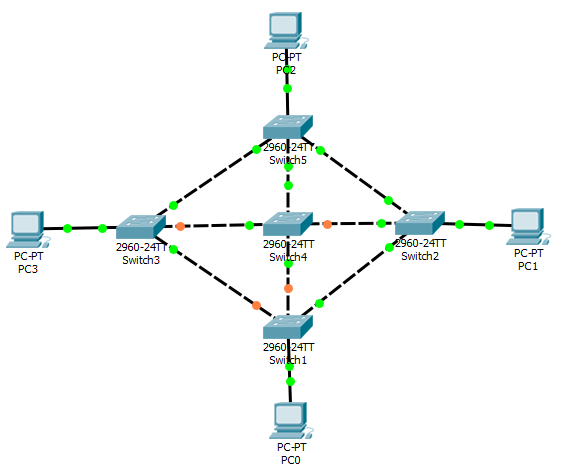
\includegraphics[height=7cm,width=8cm]{sshot-1.png}
\caption{Topología}
\label{fig:top}
\end{figure}

Primero observaremos los efectos con STP, configuraremos al Switch 2 como primario, al Switch 3 como secundario (Figura \ref{fig:config}) y con respecto a los Switchs restantes, le daremos un valor a la prioridad de cada uno de estos.(Figura \ref{fig:prio})

\begin{figure}[h!]
\centering
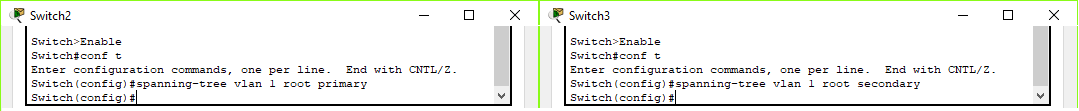
\includegraphics[height=3cm,width=15.2cm]{Primary.png}
\caption{Configuración de STP}
\label{fig:config}
\end{figure}

\newpage

\begin{figure}[h!]
\centering
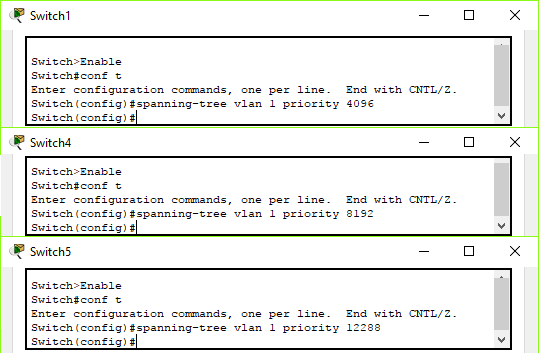
\includegraphics[height=7cm,width=10cm]{priority1.png}
\caption{Prioridad}
\label{fig:prio}
\end{figure}

Para asegurarnos de que hicimos todo correctamente, el Pc 0 le enviará un paquete al Pc 2 y como resultado tenemos una transmisión correcta y sin bucles como se observa en la Figura \ref{fig:msj1}\\

\begin{figure}[h!]
\centering
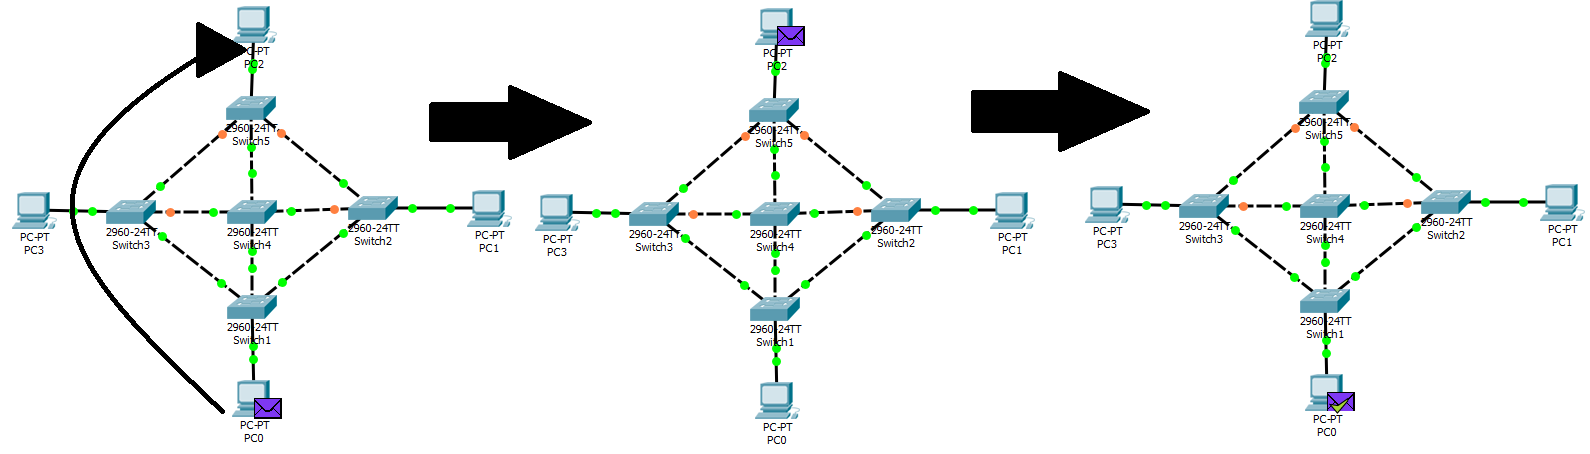
\includegraphics[height=5cm,width=13cm]{mensaje1.png}
\caption{Transmisión con STP configurado}
\label{fig:msj1}
\end{figure}

\newpage
La segunda parte de la actividad 1 es observar como sería la transmisión de datos sin el STP, así que dicho protocolo se desactivará para cada Switch dejando todos los puertos disponibles. (Figura \ref{fig:stpdes}) 

\begin{figure}[h!]
\centering
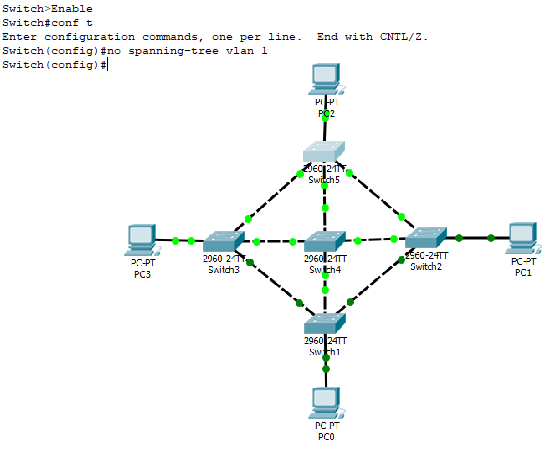
\includegraphics[height=7cm,width=10cm]{Nospanningtree.png}
\caption{STP Desactivado}
\label{fig:stpdes}
\end{figure}

Al igual que en el caso anterior el Pc 0 es el emisor y el Pc 2 es el receptor, y a los pocos momentos nos damos cuenta de que nuestro mensaje, al no tener un sólo camino, este toma todas las rutas posibles como se ve en la Figura \ref{fig:msj2}.

\begin{figure}[h!]
\centering
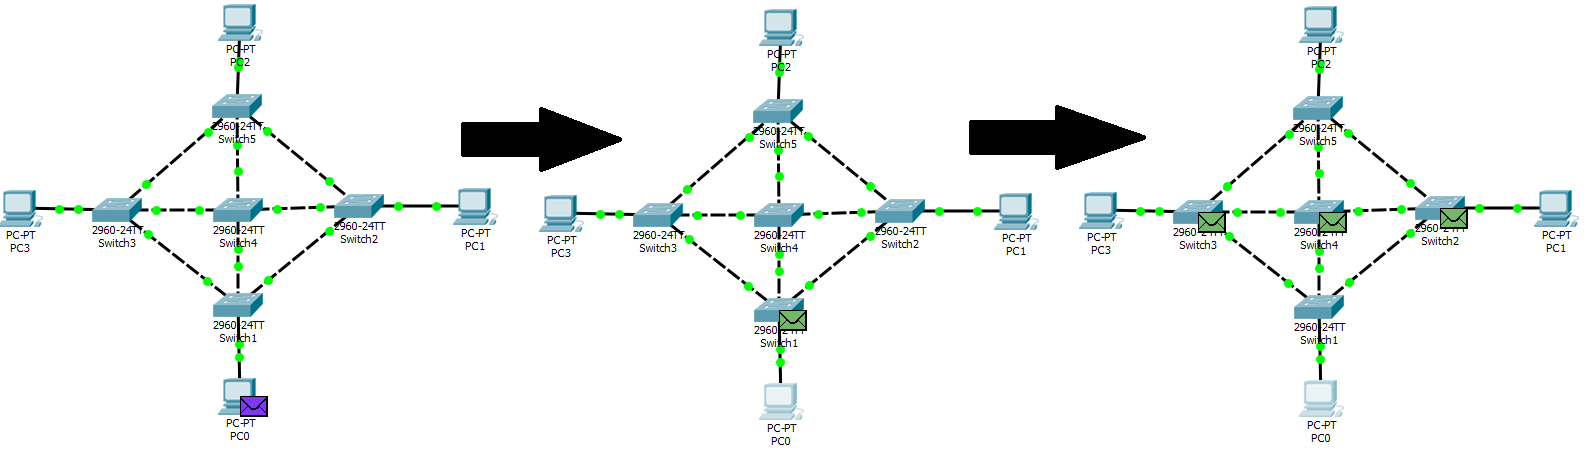
\includegraphics[height=4.5cm,width=12cm]{mensaje4.png}
\caption{STP Desactivado - Envío}
\label{fig:msj2}
\end{figure}
\newpage
Finalmente, lo que obtenemos son mensajes duplicados y dando vueltas por toda la red. Esto sin tomar en cuenta la notificación que verifica si nuestro paquete llegó correctamente. (Figura \ref{fig:msj3})
\begin{figure}[h!]
\centering
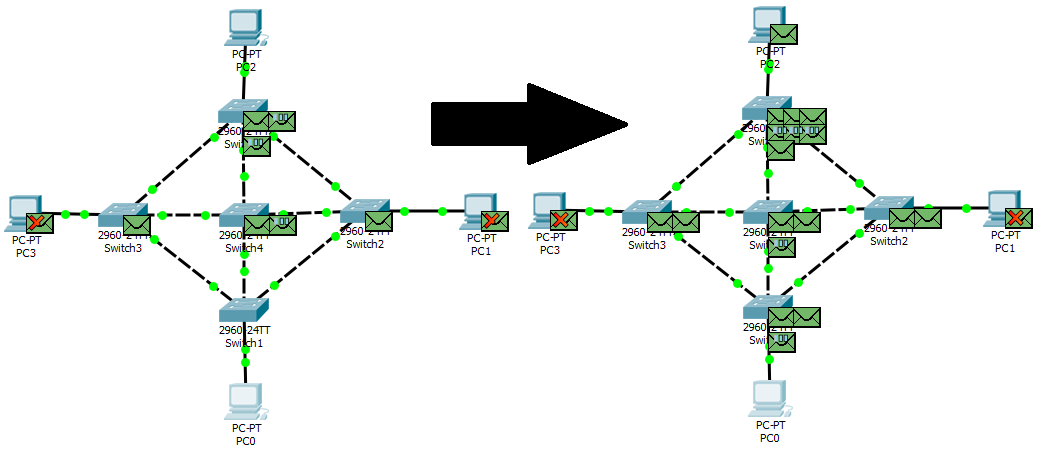
\includegraphics[height=4.5cm,width=12cm]{mensaje7.png}
\caption{STP Desactivado - Envío}
\label{fig:msj3}
\end{figure}

\newpage
\subsection{Actividad 2\vspace{0.3cm}}
Para esta actividad crearemos 4 VLANs y las implementaremos según indique el ayudante suponiendo que cada Switch esta en un piso diferente y que el computador representa una cantidad grande e indefinida de computadores y equipos conectados a la red(Figura \ref{fig:top2})

\begin{figure}[h!]
\centering
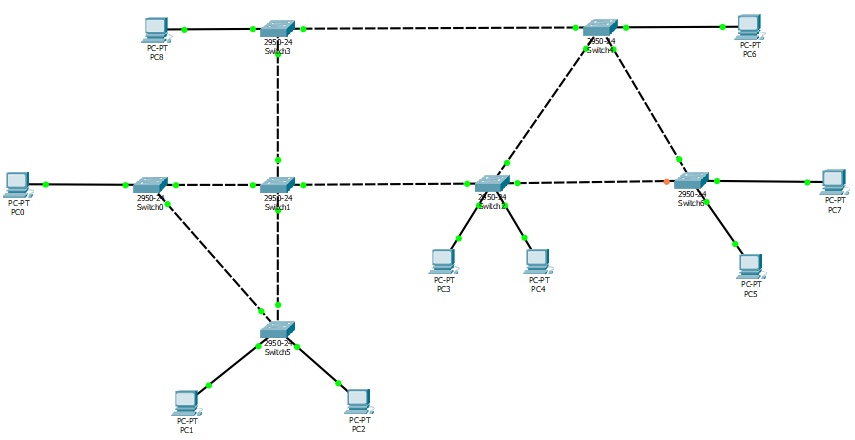
\includegraphics[height=5cm,width=12cm]{top2.png}
\caption{Topología de red - Actividad 2}
\label{fig:top2}
\end{figure}

Después de crear la topología de la Figura \ref{fig:top2} se nos pide configurar las VLAN según la siguiente tabla:\\
\newline
\begin{tabu} to 1.2\textwidth { | X[l] | X[c] | X[c] | X[c] | X[c] | X[c] | X[c] | X[c] | X[c] | X[c] |  }
 \hline
 & PC 0  & PC 1  & PC 2  & PC 3  & PC 4  & PC 5  & PC 6  & PC 7  & PC 8 \\
 \hline
 VLAN1  & X  & & & X  & & & & & &   
 \hline
 VLAN2  & & X  & & & & & & X  &  \\
 \hline
 VLAN3  & & & X  & & X  & & & & X\\
 \hline
 VLAN4  & & & & & & X  & X  & & &
 \hline
\end{tabu}
Para configurar los puertos de los Switchs se usaran los comandos dados por el ayudante:

\begin{itemize}
\item Para agregar una VLAN a un switch:\\
Switch enable\\
Switch# vlan database\\
\% Warning: It is recomm ende d to configure VLAN from config mode, as VLAN database mode is being deprecated. Please consult user documentation for configuring VTP/VLAN in config mode\\
Switch(vlan)#vlan “numerodevlan” // sin comillas y escriba la vlan que desea ingresar reemplazando numerodevlan.\\
Switch(vlan)# exit
\newpage
\item  Para agregar una puerta de red en modo Trunk:\\
Switch enable\\
Switch\# conf t\\
Enter configuration commands, one p er line. End with CNTL/Z\\
Switch(conf )\# interface fastEthernet “numero deinterfaz” // nuevamente sin comillas y número deinterfaz ya sea 0/1, 0/2, etc.\\
Switch(conf-if )\#switchport trunk allowed vlan “NUMERO”\\
Switch(conf-if )\#switchport trunk allowed vlan add “NUMERO”\\
Switch(conf-if )\#exit
\item Para agregar una puerta de red en modo Access:\\
Switch enable\\
Switch\# conf t\\
Enter configuration commands, one p er line. End with CNTL/Z\\
Switch(conf )\# interface fastEthernet “numero deinterfaz” // nuevamente sin comillas y número deinterfaz ya sea 0/1, 0/2, etc.\\
Switch(conf-if )\#switchport mode access\\
Switch(conf-if )\#switchport access vlan “NUMERO”\\
Switch(conf-if )\#exit

\end{itemize}

La topología resultante será adjuntada junto al informe y código.

\newpage
\subsection{Preguntas \vspace{0.3cm}}
\begin{itemize}
    \item ¿Cuál es la diferencia entre modo Trunk y modo Access?\\
    \newline El modo Access permite pasar solo una VLAN y casi siempre se usa para conectar dispositivos finales de las redes, el modo Trunk permite manejar el tráfico de distintas Vlan en un mismo puerto, casi siempre se utiliza para conectar 2 tipos de equipos de red como por ejemplo 2 Switchs.
    \item ¿Qué ocurre si conecto una puerta en modo Trunk a un PC?\\
    \newline Por lo que se comenta anteriormente el modo Trunk permite manejar el tráfico de distintas VLAN, por lo cual se puede decir que, si conecto una puerta en modo Trunk a un PC, este debería tener acceso a las VLAN que se asocien a esa puerta.
    \item ¿Qué ruta sigue un ping del PC 3 al PC 8? ¿Es una ruta eficiente en cuanto a tiempo? ¿Qué opción daría usted para poder llegar a los tres PC con VLAN 3 sin generar bucles y ser óptimo en tiempo?\\
    \newline
    \item ¿Qué pasa si conecto dos switchs uno con la puerta Trunk y la otra con puerta Access?\\
    \newline Debería suceder que el acceso a el switch en modo Access desde el switch en modo Trunk solo es a través de una sola VLAN , y los PCs conectados al switch en modo access solo deberían estar conectados a esa misma VLAN.
    \item ¿Cuáles son las ventajas de este sistema llamado VLAN? Mencione al menos 3
     \begin{enumerate}
        \item Mayor flexibilidad en la administración y en los cambios de red, ya que permite cambiar la arquitectura de la red fácilmente.
        \item Mayor seguridad, ya que se mantiene la información en la Vlan designada y no se puede acceder de otra Vlan.
        \item Disminuye la transmisión de tráfico en la red.
    \end{enumerate}
\end{itemize}
\newpage
\section{Conclusión\vspace{0.5cm}}

Tanto la importancia del STP como la del VLAN se vieron reflejadas en este laboratorio puesto que, con la ausencia de alguno de ellos, el proceso de transmisión de datos sería mucho más complicado y caótico. Por otra parte, la presencia de estos elementos nos permiten disminuir los errores posibles en nuestras redes y abaratar costos que jamás esta demás.

\end{document}
